\documentclass[../../../../main.tex]{subfiles}
\begin{document}

\begin{flushright}
\footnotesize\textit{【自動文字起こし・要確認】}
\end{flushright}

\begin{proof}[解]
\begin{center}
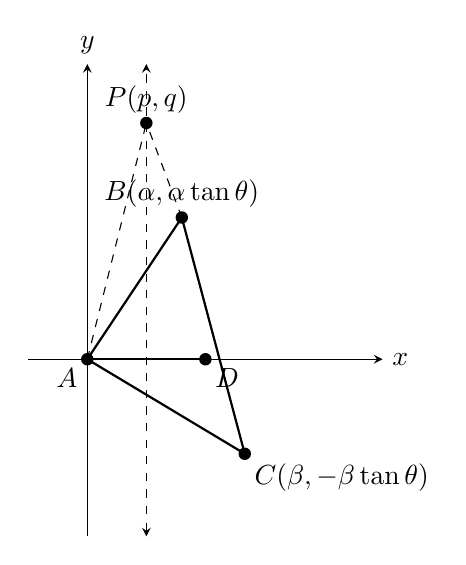
\begin{tikzpicture}[scale=1.5, >=stealth]
  \draw[->] (-0.5,0) -- (2.5,0) node[right] {$x$};
  \draw[->] (0,-1.5) -- (0,2.5) node[above] {$y$};
  \node[below left] at (0,0) {$A$};
  \coordinate (A) at (0,0);
  \coordinate (D) at (1,0);
  \node[below right] at (1,0) {$D$};
  
  \coordinate (B) at (0.8, 1.2);
  \coordinate (C) at (1.333, -0.8);
  \coordinate (P) at (0.5, 2.0);
  
  \draw[line width=0.8pt] (A) -- (B) -- (C) -- cycle;
  \draw[line width=0.8pt] (A) -- (D);
  \draw[dashed] (B) -- (P);
  \draw[dashed] (A) -- (P);
  \draw[<->, dashed] (0.5,-1.5) -- (0.5,2.5);
  
  \node[above] at (B) {$B(\alpha, \alpha\tan\theta)$};
  \node[below right] at (C) {$C(\beta, -\beta\tan\theta)$};
  \node[above] at (P) {$P(p,q)$};
  
  \fill (A) circle (1.5pt);
  \fill (D) circle (1.5pt);
  \fill (B) circle (1.5pt);
  \fill (C) circle (1.5pt);
  \fill (P) circle (1.5pt);
\end{tikzpicture}
\end{center}

$AD=1$ として一般性を失わない．A を原点とし，AD を $x$ 軸とする上図のような座標平面をとり
\[
  B(\alpha, \alpha \tan \theta) \quad \left(0 < \theta < \frac{\pi}{2}\right)
\]
\[
  C(\beta, -\beta \tan \theta)
\]
とおく ($\alpha \neq \beta$, $\alpha, \beta > 0$)．
\begin{align*}
  BC: &(\beta + \alpha)\tan \theta \cdot (x - \alpha) + (\beta - \alpha)(y - \alpha \tan \theta) = 0 \\
  &(\beta + \alpha)\tan \theta \cdot x + (\beta - \alpha)y - 2\alpha\beta \tan \theta = 0 \quad \dots \text{①}
\end{align*}
これが $D(1,0)$ を通るので
\[
  (\beta + \alpha)\tan \theta = 2\alpha\beta \tan \theta
\]
$\tan \theta \neq 0$ より
\[
  \alpha + \beta = 2\alpha\beta \quad \dots \text{②}
\]

$\triangle ABC$ の外心 $O'(X,Y)$ とすると，$O'A = O'B = O'C$ から
\begin{align}
  X &= \frac{1}{4}(\tau^2 + 1)(\alpha + \beta) \quad \dots \text{③} \quad (\tau = \tan \theta) \\
  Y &= \frac{1}{4\tau}(\tau^2 + 1)(\alpha - \beta) \quad \dots \text{④}
\end{align}
となり，外接円は $C: (x-X)^2 + (y-Y)^2 = X^2 + Y^2$ だから点 A での接線 $l$ は
\begin{align*}
  l: &Xx + Yy = 0 \\
  &(\alpha + \beta)\tau x + (\alpha - \beta)y = 0 \quad \dots \text{⑤}
\end{align*}

よって ①, ⑤ から BC と $l$ の交点 $P(p,q)$ は
\[
  p = \frac{1}{2}, \quad q = \frac{\alpha + \beta}{\beta - \alpha} \frac{\tau}{2}
\]
よって P は定直線 $x = \dfrac{1}{2}$ 上にあるから示された．

\bigskip
\begin{proof}[別解]
\begin{center}
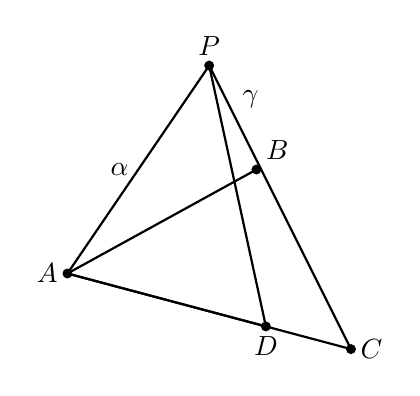
\begin{tikzpicture}[scale=1.2, >=stealth]
  \coordinate (P) at (1.5, 3.0);
  \coordinate (A) at (0, 0.8);
  \coordinate (C) at (3.0, 0);
  \coordinate (B) at (2.0, 1.9);
  \coordinate (D) at (2.1, 0.24);
  
  \draw[line width=0.8pt] (A) -- (P) -- (C) -- cycle;
  \draw[line width=0.8pt] (A) -- (B);
  \draw[line width=0.8pt] (P) -- (D);
  \draw[line width=0.8pt] (A) -- (D);
  
  \node[above] at (P) {$P$};
  \node[left] at (A) {$A$};
  \node[right] at (C) {$C$};
  \node[above right] at (B) {$B$};
  \node[below] at (D) {$D$};
  
  \node[left] at (0.75, 1.9) {$\alpha$};
  \node[above right] at (1.75, 2.45) {$\gamma$};
  
  \fill (A) circle (1.5pt);
  \fill (B) circle (1.5pt);
  \fill (C) circle (1.5pt);
  \fill (D) circle (1.5pt);
  \fill (P) circle (1.5pt);
\end{tikzpicture}
\end{center}

$AP = \alpha$, $AB = \beta$, $BP = \gamma$ とおく．
$\triangle ABP \sim \triangle CAP$ より
\[
  AC = \frac{\alpha}{\gamma}\beta \quad \dots \text{①}
\]
又，$\alpha^2 = \gamma \cdot PC$ から
\[
  PC = \frac{\alpha^2}{\gamma} \quad \dots \text{②}
\]
従って
\[
  BD = BC \cdot \frac{AB}{AB+AC} = \left(\frac{\alpha^2}{\gamma} - \gamma\right) \frac{\beta}{\beta + \frac{\alpha}{\gamma}\beta} = \alpha - \gamma
\]
から $DP = PB + BD = \gamma + (\alpha - \gamma) = \alpha$ だから $\triangle APD$ は 2 等辺三角形．
よって P は AD の垂直2等分線上にある．
\end{proof}
\end{proof}

\newpage

\end{document}
